\documentclass[titlepage]{article}
\usepackage{amsfonts}
\usepackage{bbm}
\usepackage{graphicx}
\renewcommand{\baselinestretch}{1}
\usepackage[utf8]{inputenc}
\usepackage{color}
\usepackage[T1]{fontenc}
\usepackage{geometry}
\usepackage{amsmath}
\usepackage{enumerate}
\usepackage{caption}
\usepackage{graphicx}
\usepackage{subcaption}
\usepackage{array}
\usepackage{fullpage}
\usepackage{algorithm2e}
\usepackage{float}
\usepackage{listings}
\usepackage{tikz}
\usepackage{amssymb}

\everymath{\displaystyle}
\newtheorem{theorem}{Theorem}[section]
\newtheorem{lemma}[theorem]{Lemma}
\newtheorem{proposition}[theorem]{Proposition}
\newtheorem{corollary}[theorem]{Corollary}

\newcommand{\argmin}{\operatornamewithlimits{argmin}}

\newenvironment{proof}[1][Proof]{\begin{trivlist}
\item[\hskip \labelsep {\bfseries #1}]}{\end{trivlist}}
\newenvironment{definition}[1][Definition]{\begin{trivlist}
\item[\hskip \labelsep {\bfseries #1}]}{\end{trivlist}}
\newenvironment{example}[1][Example]{\begin{trivlist}
\item[\hskip \labelsep {\bfseries #1}]}{\end{trivlist}}
\newenvironment{remark}[1][Remark]{\begin{trivlist}
\item[\hskip \labelsep {\bfseries #1}]}{\end{trivlist}}

\newcommand{\qed}{\nobreak \ifvmode \relax \else
      \ifdim\lastskip<1.5em \hskip-\lastskip
      \hskip1.5em plus0em minus0.5em \fi \nobreak
      \vrule height0.75em width0.5em depth0.25em\fi}


\begin{document}
\title{Coach Ranking Model}
\author{Akilesh Potti, Dominick Twitty, Wenhai Yang}
\maketitle

\begin{abstract}
Todo
\end{abstract}



\noindent\textbf{Disclaimer:} For legal and moral reasons, all geographical locations and company names used in this paper are entirely fictional unless otherwise stated. However, for the sake of accuracy, real world data was used to tune our model.


\section{The Problem}
\begin{enumerate}
\item Todo
\end{enumerate}


\section{Model assumptions}
\begin{enumerate}
\item Todo
\end{enumerate}

\section{Models}

\subsection{Simple Heuristic Model}
\subsubsection{Sorting by Win/Loss Ratio}
\subsubsection{Sorting by Net Wins}
\subsubsection{Differentiate between Games}


\subsection{Graphical Model}
It comes very natural for us to consider the problem as a graph. The nodes of the graph are the coaches. An edge between two nodes denotes the relation between two coaches, such as the game result of them playing against each other.
\\

\noindent This idea of representing the problem as a graph is a very good step forward because it allow us to go beyond the simple statistics like win/loss ratio of a single coach, and gain more insight from the data.
\\

\noindent Another advantage of this model is that it can aggregate data from different time periods. For example if coach A beats coach B and then retired in 1990, and coach B beat coach C later in 1995, then in the graph we will have a way to compare coach A and coach C because there is a path from A to C through B, even though they never played against each other.

\subsubsection{Topolical Ordering}
A very first idea that comes to mind is Topological Ordering. In this sub-model, there exist an edge from $i$ to $j$ if and only if among all the games $i$ played against $j$, $j$ beat $i$ more often than $i$ beat $j$ (net-loss). Then if there exists a Topological Ordering of the graph, we have a ranking of the coaches based on their rival history.
\\

\noindent Consider the following example. Coach 1 has been beaten by both 2 and 3, coach 2 has been beaten by coach 3 and 4, coach 3 has been beaten by coach 4, and coach 4 is never beaten by anyone. We have a topological ordering in the graph: $\{1, 2, 3, 4\}$, and it is natural to conclude that coach 4 is the best coach among them. (For now, when we talk A is beaten by B, we mean net-loss, which means A is beaten by B more often than B is beaten by A. We will introduce more sophisticated measures later).

\begin{center}
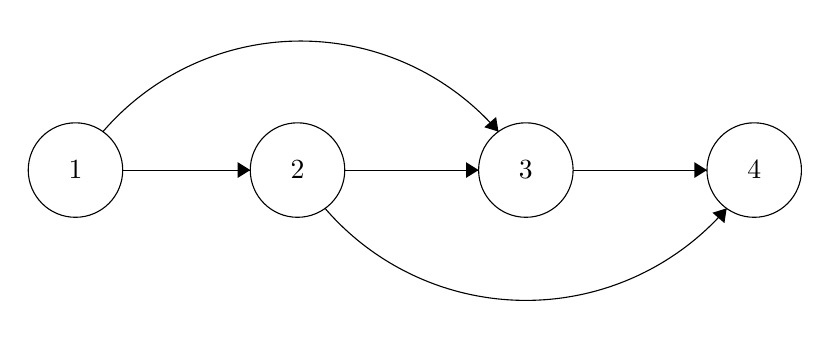
\begin{tikzpicture}[scale=0.2]
\tikzstyle{every node}+=[inner sep=0pt]
\draw [black] (16.1,-27.9) circle (3);
\draw (16.1,-27.9) node {$1$};
\draw [black] (30.2,-27.9) circle (3);
\draw (30.2,-27.9) node {$2$};
\draw [black] (44.7,-27.9) circle (3);
\draw (44.7,-27.9) node {$3$};
\draw [black] (59.2,-27.9) circle (3);
\draw (59.2,-27.9) node {$4$};
\draw [black] (19.1,-27.9) -- (27.2,-27.9);
\fill [black] (27.2,-27.9) -- (26.4,-27.4) -- (26.4,-28.4);
\draw [black] (33.2,-27.9) -- (41.7,-27.9);
\fill [black] (41.7,-27.9) -- (40.9,-27.4) -- (40.9,-28.4);
\draw [black] (47.7,-27.9) -- (56.2,-27.9);
\fill [black] (56.2,-27.9) -- (55.4,-27.4) -- (55.4,-28.4);
\draw [black] (17.843,-25.463) arc (139.24738:40.75262:16.577);
\fill [black] (42.96,-25.46) -- (42.81,-24.53) -- (42.06,-25.18);
\draw [black] (57.453,-30.334) arc (-40.77401:-139.22599:16.84);
\fill [black] (57.45,-30.33) -- (56.55,-30.61) -- (57.31,-31.27);
\end{tikzpicture}
\end{center}

\noindent However, one natural limitation of this model is the following theorem:

\begin{theorem}
A graph $G$ has a topological ordering if and only if it is a DAG (directed acyclic graph).
\end{theorem}
\begin{proof}
See Section 3.6 of Algorithms Design by Kleinberg and Tardos.
\end{proof}

\noindent To solve this issue, we think of two algorithms. One is to reduce the originial graph into a DAG: keep removing the most "unimportant" edges untils the graph is acyclic. By most "unimportant" we then have to find a way to measure the importance of an edge. In this model, the weight (or importance) an edge by the net-loss it is associated with:

$$w(e_{i, j}) = \mbox{number of times j beats i} - \mbox{number of times j beats i}$$

\noindent The algorithm then works as following:

\vspace{5mm}

\begin{algorithm}[H]

\While{$G$ is not DAG}{
$e_{min} = \argmin_{e \in E} w(e)$\;
Remove $e_min$ from $G$
}

\end{algorithm}

\vspace{5mm}

\noindent However, this algorithm has apparent flaws: suppose even though coach A and coach B only encounter each other once, however it is in the SuperBowl, while the matchup between coach A and coach C is quite often but only in friendly games or early-season games and therefore the result is less important and less indicative of their comparative abilities. Therefore using the net-loss as the only measurement of the importance of an edge can possibly remove the important edge and keep the unimportant ones. We can of course tweak the edge-weight by introducing the importance of a game, the time in both coaches' career when the match happens, etc., but simply adding heuristics seem not like the best approach to the problem.
\\

\noindent The second algorithm requires a certain "leap of faith" by introducing randomness into our model:

\subsubsection{Markov Chain (Voting Model)}

To solve the problem of Topogical Ordering, instead of trying to create a DAG to fit the algorithm, we decide adjust the mechanism behind ranking using Topological Ordering.
\\

\noindent Imagine instead of having us, the spectators doing the voting and the ordering, each coach will have a $\bf{vote}$ of a certain $\bf{size}$, which she can divide up into pieces. She can then give the chunks of the vote to different coaches which she think is definitely better coach than she is. We assume the coaches to be rational: she doesn't take into account the opinions of amateurs and public media, and only give out votes to the one she truly believe is better than her (one possible way is only give out vote to the coaches who has beaten her). Then we will rank the coaches based on how many votes each coach eventually get. However since the coaches form a graph and there even might be cycles in the game, so at each timestep a coach can be both receiving and giving. What we are interested in is the distribution of the votes at some large time.
\\

\noindent Consider the following example. There are four coaches: 1, 2, 3, 4. Coach 1 has been beaten by 1 and 4, coach 2 has been beaten by 3 and 4, coach 3 has been beaten by 4 and 1, coach 4 has never been beaten.

\begin{center}
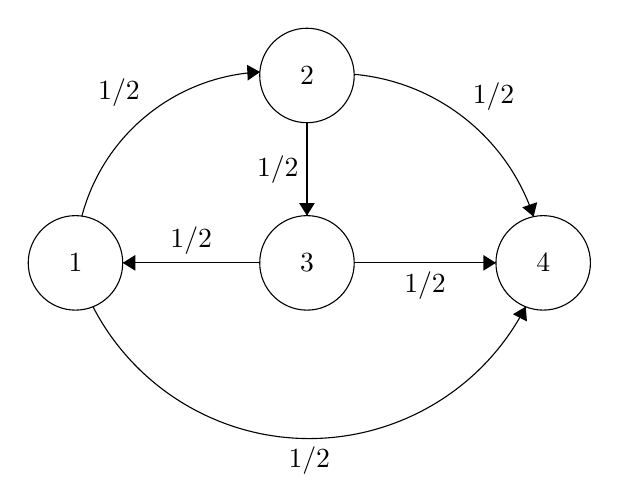
\begin{tikzpicture}[scale=0.2]
\tikzstyle{every node}+=[inner sep=0pt]
\draw [black] (37.8,-30.2) circle (3);
\draw (37.8,-30.2) node {$3$};
\draw [black] (23.1,-30.2) circle (3);
\draw (23.1,-30.2) node {$1$};
\draw [black] (37.8,-18.3) circle (3);
\draw (37.8,-18.3) node {$2$};
\draw [black] (52.8,-30.2) circle (3);
\draw (52.8,-30.2) node {$4$};
\draw [black] (51.691,-32.982) arc (-27.29025:-152.70975:15.462);
\fill [black] (51.69,-32.98) -- (50.88,-33.46) -- (51.77,-33.92);
\draw (37.95,-41.86) node [below] {$1/2$};
\draw [black] (23.506,-27.235) arc (165.22297:92.75902:12.309);
\fill [black] (34.82,-18.08) -- (33.99,-17.62) -- (34.04,-18.62);
\draw (25.86,-20.31) node [above] {$1/2$};
\draw [black] (40.793,-18.226) arc (84.9222:18.22552:13.234);
\fill [black] (52.19,-27.27) -- (52.42,-26.35) -- (51.47,-26.67);
\draw (49.65,-20.55) node [above] {$1/2$};
\draw [black] (34.8,-30.2) -- (26.1,-30.2);
\fill [black] (26.1,-30.2) -- (26.9,-30.7) -- (26.9,-29.7);
\draw (30.45,-29.7) node [above] {$1/2$};
\draw [black] (40.8,-30.2) -- (49.8,-30.2);
\fill [black] (49.8,-30.2) -- (49,-29.7) -- (49,-30.7);
\draw (45.3,-30.7) node [below] {$1/2$};
\draw [black] (37.8,-21.3) -- (37.8,-27.2);
\fill [black] (37.8,-27.2) -- (38.3,-26.4) -- (37.3,-26.4);
\draw (37.3,-24.25) node [left] {$1/2$};
\end{tikzpicture}
\end{center}

\noindent The Markov Chain above shows how the vote will be given out at each timestep: coach 1 will give out half of her vote to coach 2 and the other half to 3, coach 2 will give out half of her vote to coach 3 and the other half to coach 4, coach 3 will give out half of her vote to coach 1 and the other half to coach 4. Coach 4, since she never lost to anyone, will simply keep her vote to herself. We can therefore see this can be modeled as a Markov Chain, and the distribution of votes at some large time is the stationary probability distribution of this Markov Chain:

$$ \pi = \phi_{0} P^n \mbox{ for some initial distribution } \phi_{0}$$

\noindent where $\bf{P}$ is the probability transition matrix, with $\bf{P}_{i,j}$ equal to the proporption of her chunk coach i will give to j (can also be interpreted as the probability of going from i to j in the Markov Chain):

\[
\bf{P} = 
\begin{bmatrix}
0 & 0.5 & 0.5 & 0 \\
0 & 0 & 0.5 & 0.5 \\
0.5 & 0 & 0.5 & 0 \\
0 & 0 & 0 & 1
\end{bmatrix}
\]

\noindent We know that if the Markov Chain is irreducable and aperiodic, then such a stationary distribution exists, and is unique, and it is the left eigenvector of $\bf{P}$ for the eigenvalue 1.


\subsubsection*{Irreducable \& Aperiodic}

\noindent Apparently, the example we show doesn't satisfy the property. To make sure the matrix we encounter will be irreducable and aperiodic, we use a similar technique as the PageRank algorithm used by Google:

\begin{enumerate}
\item For dead-ends (coach 4 in the example), in each step she will split her vote into equal pieces and give one piece to every coach, (go to a random state in the Markov Chain)
\item For non-deadends (coach 1, 2, 3 in the example), in each step with he will first split her vote into two, with proportion $\alpha$ and $1 - \alpha$. With the $\alpha$ proportion she did what she did before, spliting it and give the pieces to coaches who have beaten her, the remaining $1 - \alpha$ she will split into equal pieces and give one piece to every coach.
\end{enumerate}

\noindent Therefore, after adjusting for deadends in ${\bf P}$, the new probability transition matrix can be represented as:

$${\bf D} = \alpha {\bf P} + (1 - \alpha) {\bf U}$$

\noindent where $\bf{U}$ with all entries equal to $\frac{1}{n}$, $n$ being the total number of coaches (or number of states in the Markov Chain).
\\

\noindent With the new probability transition matrix, since all entries in $\bf{D}$ are positive, we know by Perron-Frobenius theorem that $\bf{D}$ is both irreducable and aperiodic, and that the stationary distribution $\pi$ exists and is unique. With $\pi$ we can find the coaches with the top $5$ probability and they will be the best coaches "of all time" since they get the most proportion of votes from all coaches in the long-run.

\subsubsection*{Formal Representation}

$$G(V, E) \mbox{ represents the graph of coaches}$$
$$V = \{v_1, v_2 ... v_n\} \mbox{ where } v_i \mbox{ is coach i }$$
$$(v_i, v_j) \in E : \mbox{ coach j beats coach i more often than coach i beats coach j }$$

\[
    {\bf D} (i, j)= 
\begin{cases}
    \alpha \frac{ I\{(v_i, v_j) \in E\}}{d(v_i)} + (1-\alpha)\frac{1}{n},& \text{if } d(v_i) \geq 1\\
    \frac{1}{n},              & \text{otherwise}
\end{cases}
\]


\subsubsection*{Efficient Implementation}

Since the matrix ${\bf D}$ is huge and all entries are non zero, calculating its eigenvalues and eigenvectors directly can be very inefficient computationally. However ${\bf P}$ is a sparse matrix and most of its entries are zero. To make sure we will be able to produce the eigenvector that represents the stationary distribution efficiently, we use Power Method:

\vspace{5mm}

\begin{algorithm}[H]

$v = (1/n, ... ,1/n)$\;
\While{$\| \alpha v {\bf P} + (1 - \alpha)(1, ... ,1) - v\| < e^{-8}$}{
$v = \alpha v {\bf P} + (1 - \alpha)(1, ... ,1)$\;
}
\Return $v$\;
\end{algorithm}

\vspace{5mm}

\noindent Since $v {\bf P}$ can be calculated using sparse matrix ${\bf P}$, this algorithm is much more computationally efficient than simply calculating the eigenvectors of ${\bf D}$. As $\alpha$ increases, the time it takes for $v$ to converge is shorter, but the difference in the ranking might be less significant, therefore this is a tradeoff and we pick $\alpha = 0.95$.

\subsubsection*{More on Edge Weights}

\noindent In the model we introduced above, in situation where $d(v_i) \geq 1$ (which is something we assume in the rest of this section), ${\bf P}(i, j) = \frac{ I\{(v_i, v_j) \in E\}}{d(v_i)}$, where $I\{(v_i, v_j) \in E\}$ is simply an indicator variable indicating whether i has a net-loss against j. However there are a lot more information we can capture, if we think more about the vote coach i will give:

\begin{enumerate}
\item Game's importance: The more important the game is, the more effort both coaches will put in, and therefore the game result will be more convincing and informative, and more likely coach $i$ will be to give the vote to coach $j$, had coach $i$ lost.
\item Time in Career: If it is early in the career of coach $i$ when he lost to coach $j$, she is going to put less weight than the game she lost later in her career, since it is typical for a coach to learn from failure early and become a better coach later. Therefore coach $i$ will be more convinced to give vote to someone she lost to later in her career.
\item Game Score: A game lost very close is definitely less convincing than a game entirely dominated by opponent. Therefore the more score coach $i$ lost, the more convinced she will be to give your vote to your opponent.
\end{enumerate}

\noindent There are definitely more information that can be informative, however due to the difficulty of data-mining and significance comparison, we come up with the following updated formula to calculate the weight for edge weight:
\\

\noindent Let $T$ be the set of all games, $C: T \rightarrow \mathbb{R}$ map a game to the score difference of the game (positive winning score, 0 if draw), .
$$ T_{i,j} = \{t \in T : \mbox{ coach i lost to coach j in } t\} $$
$$ C $$
$$w(v_i, v_j) = \sum$$


\subsection{Machine Learning Model}



\section{Results, Validation, and Robustness}


$$p_{unreg} = k \ln (t_{reg})$$
$$\frac{p_{unreg'}}{p_{unreg}}  = \frac{\ln_{t_{reg}}}{ \ln{t_{reg'}}}$$

\begin{center}
\begin{tabular}{ | c | c | c | c | c | c | c | c | c | }
\hline
 Number of Cabs & 14 & 15 & 16 & 17 & 18 & 19 & 20 & 21 \\\hline
Uni Ind/Conglo & 1.5720  &  1.3773  &  1.2880 &   1.2071 &   1.1932 &  1.2113  &  1.1201  &  1.0672\\\hline
Prop Ind/Conglo & 1.6876  &  1.4040  &  1.2459  &  1.1248  &  1.2558  &  1.1498  &  1.1033  &  1.1022\\\hline
Disprop Ind/Conglo & 2.1519  &  2.0706 &   2.0489  &  1.9399  &  1.8725 &   1.8174  &  1.6990 &   1.3905\\
\hline
\end{tabular}
\end{center}

\section{Strengths and Weaknesses}
\subsection{Strengths}
\begin{itemize}
\item Todo
\end{itemize}
\subsection{Weaknesses}
\begin{itemize}
\item Todo
\end{itemize}

\section{Conclusions}
Todo

\section{Future work}
\begin{itemize}
\item Todo
\end{itemize}

\pagebreak

\section{Bibliography}
\begin{thebibliography}{9}

\bibitem{OSM} OpenStreetMaps API,
\verb|http://www.openstreetmap.org/#map=14/42.4427/-76.4984|
\bibitem{Gist} Github Gist by user aflaxman,
\verb|https://gist.github.com/aflaxman/287370/|
\bibitem{Re} $\text{A stochastic optimization model for real-time ambulance redeployment}$,
\\\verb|http://www.sciencedirect.com/science/article/pii/S0305054813000385|
\bibitem{Ithaca} Ithaca Demographics,
\verb|http://www.ci.ithaca.ny.us/maps/index.cfm|
\bibitem{Cornell} Cornell Demographics,
\verb|http://www.cornell.edu/about/facts/stats.cfm|
\bibitem{IC} Ithaca College,
\verb|http://www.ithaca.edu/admission/facts/|


\end{thebibliography}

\pagebreak

\section{Code}


\definecolor{mygreen}{rgb}{0,0.6,0}
\definecolor{mygray}{rgb}{0.5,0.5,0.5}
\definecolor{mymauve}{rgb}{0.58,0,0.82}

\lstset{ %	
  backgroundcolor=\color{white},   % choose the background color; you must add \usepackage{color} or \usepackage{xcolor}
  basicstyle=\footnotesize,        % the size of the fonts that are used for the code
  breakatwhitespace=false,         % sets if automatic breaks should only happen at whitespace
  breaklines=true,                 % sets automatic line breaking
  captionpos=b,                    % sets the caption-position to bottom
  commentstyle=\color{mygreen},    % comment style
  deletekeywords={...},            % if you want to delete keywords from the given language
  escapeinside={\%*}{*)},          % if you want to add LaTeX within your code
  extendedchars=true,              % lets you use non-ASCII characters; for 8-bits encodings only, does not work with UTF-8
  frame=single,                    % adds a frame around the code
  keepspaces=true,                 % keeps spaces in text, useful for keeping indentation of code (possibly needs columns=flexible)
  keywordstyle=\color{blue},       % keyword style
  morekeywords={*,...},            % if you want to add more keywords to the set
  numbers=left,                    % where to put the line-numbers; possible values are (none, left, right)
  numbersep=5pt,                   % how far the line-numbers are from the code
  numberstyle=\tiny\color{mygray}, % the style that is used for the line-numbers
  rulecolor=\color{black},         % if not set, the frame-color may be changed on line-breaks within not-black text (e.g. comments (green here))
  showspaces=false,                % show spaces everywhere adding particular underscores; it overrides 'showstringspaces'
  showstringspaces=false,          % underline spaces within strings only
  showtabs=false,                  % show tabs within strings adding particular underscores
  stepnumber=2,                    % the step between two line-numbers. If it's 1, each line will be numbered
  stringstyle=\color{mymauve},     % string literal style
  tabsize=2,                       % sets default tabsize to 2 spaces
  title=\lstname,                  % show the filename of files included
  columns=fullflexible,basicstyle=\ttfamily,  
  language=Python    
}
\begin{lstlisting}[frame=none]
\end{lstlisting}

\end{document}